\autoref{fig:bearing_fh_tm} shows that the \ac{TM} can be positioned at various distances and angles in relation to the \ac{FH}.
For one corn harvest scenario, \textcite{klingler_agriculture_2018} found out that the \ac{RSS} can drop due to
shadowing effects caused by the size and shape of the \ac{FH} and the \ac{TM}.

In a field experiment, I want to analyze which positions of the \ac{TM} and \ac{FH} cause the shadowing effects which
subsequently reduce the \ac{RSS}, and how physical layer parameters like \ac{MCS} and \ac{STBC} can used to ensure a low
\ac{PER}.

For the experiment, I will use a \ac{CH} instead of a \ac{FH} as it has a similar shape and size as a \ac{FH} and is available.
The \ac{TM} will be a Tractor pulling a trailer of the type HW80.
Both machines will be equipped with a \ac{GPS} receiver and Wi-Fi devices which record the position, \ac{RSS} and the \ac{PER} of the
exchanged packets.
The \ac{CH} will be positioned in an agricultural field.
The tractor will start \SI{50}{\metre} behind the \ac{CH}, advance to the \ac{CH} and pass the \ac{CH} slowly with a
speed of \SIrange{1}{5}{\kilo\metre\per\hour} (\SIrange{0.28}{1.39}{\metre\per\second}) as shown in \autoref{fig:fieldDrive}.
\begin{figure}[]%
	\centering
	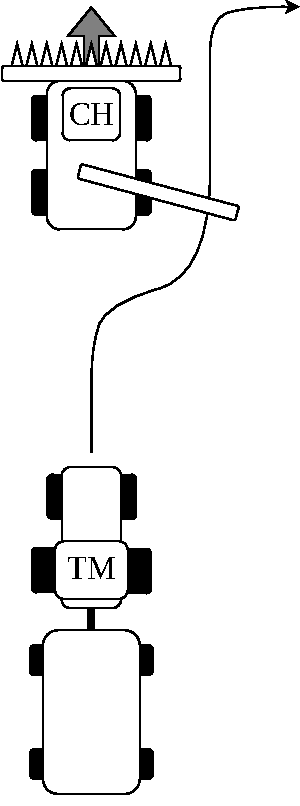
\includegraphics[width=0.2\textwidth]{figures/FieldExperimentDrive}
	\caption{Path around the static \acf{CH}, which the \acf{TM} will drive during the experiment to mimic various overloading positions}%
	\label{fig:fieldDrive}
\end{figure}
While driving along the specified path, the tractor will mimic various overloading positions, where shadowing effects can occur. After the tractor has passed the \ac{CH},
it will drive back to its starting position, and the experiment will be repeated with different overloading distances between the \ac{CH} and the tractor.

During the experiments, \ac{GPS} receivers at the agricultural machines will record the position and speed of the machines every \SI{1}{\second}.

The Wi-Fi setup consists of a Milesight Industrial Router UR75 \footnote{\url{https://iot-shop.de/en/shop/mil-ur75-500gl-g-p-w-milesight-ur75-500gl-g-p-w-industrial-cellular-5g-router-with-gps-wifi-and-poe-5677}}, which implements the standards IEEE 802.11 b/g/n in the \SI{2.4}{\giga\hertz} band and IEEE 802.11 a/n/ac in the \SI{5}{\giga\hertz} band and
IEEE 802.11 a/n/ac in the \SI{5}{\giga\hertz} band.
The router is equipped with two omnidirectional antennas for  \SI{2.4}{\giga\hertz} and \SI{5}{\giga\hertz} usage.
\textcite{brinkhoff_characterization_2017} and \textcite{paul_characterizing_2011}  already found out that placing the antenna higher above ground improves
the robustness and communication range of Wi-Fi networks in an outdoor environment.
As the regulation in the German Law StVZO §32 Abs. 2 limits the height of
every agricultural vehicle or combination of vehicles to less than \SI{4.0}{\metre}, the maximum antenna height is \SI{4}{\metre} above the ground. Therefore, I will mount the router on the tractor's roof at a height \SI{4}{\metre} above the ground.

I set up two Wi-Fi devices on the \ac{CH}, which are two UP Squared Boards \footnote{\url{https://eu.mouser.com/datasheet/2/826/UP_Square_DatasheetV0_4-3084829.pdf}} with an Intel AX210 Wi-Fi module \footnote{\url{https://docs.alfa.com.tw/datasheets/alfa-network_ait-ax210-ex_latest.pdf}}.

Every Intel AX210 Wi-Fi module supports the IEEE 802.11ax standard for \SI{2.4}{\giga\hertz}, \SI{5}{\giga\hertz} and \SI{6}{\giga\hertz} band and is equipped with two antennas,
which support omnidirectional transmissions in the \SI{2.4}{\giga\hertz}, \SI{5}{\giga\hertz} and \SI{6}{\giga\hertz} band and have a gain of \SI{5}{\decibel}.
The boards are mounted on the roof of the \ac{CH} next to one another at a height \SI{4}{\metre} above the ground too.

The router on the tractor sets up a Wi-Fi \ac{AP}.
One of the boards on the \ac{CH} connects to the \ac{AP} of the router as a Wi-Fi \ac{STA} and hosts an iperf3 \footnote{\url{https://iperf.fr/}} server.
A notebook is connected via LAN to the router and runs an iperf3 client, which connects to the iperf3 server on the \ac{CH}.
The iperf3 client sends \SI{100}{\byte} \ac{UDP} packets every \SI{100}{\milli\second} to the iperf3 server on the \ac{CH}.
The server records the received packets.

Many different Wi-Fi transmissions arise through the iperf3 \ac{UDP} packets, the Wi-Fi manager of the Milesight Industrial Router, and the Intel AX210 Wi-Fi card.
These transmissions can be RTS/CTS, ACK, Data, Beacon or Probe request frame, displayed in \autoref{fig:fieldWifi}.
Through testing, I found out that the Wi-Fi manager of the Wi-Fi devices can apply VHT \ac{MCS} \numrange{0}{9} and \ac{STBC} as physical layer configurations.

\begin{figure}[H]%
	\centering
	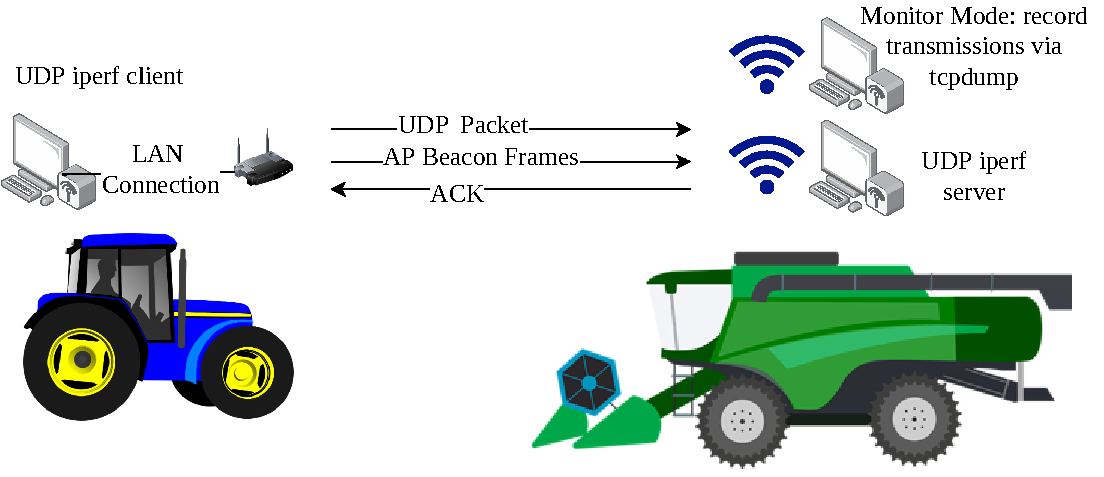
\includegraphics[width=0.8\textwidth]{figures/FieldExperimentwifi}
	\caption{Wi-Fi transmissions between the Wi-Fi \ac{AP} on the \acf{TM} and the Wi-Fi \ac{STA} on the \acf{CH}, which
	are recorded by a third Wi-Fi device in monitor mode on the \ac{CH}}
	\label{fig:fieldWifi}%
\end{figure}

The other UP Squared Board on the \ac{CH} uses the Wi-Fi card in the monitor mode and records every transmission in the \SI{5.6}{\giga\hertz} band using tcpdump \footnote{\url{https://www.tcpdump.org/}}.
Since the UP Squared board is placed next to the other board on the roof of the \ac{CH}, it can record the same signals the other board receives in the \ac{UDP} transmission.
The tcpdump records are in pcap - format, which can be analyzed using Wireshark\footnote{\url{https://www.wireshark.org/}}.
Using Wireshark, I can identify possible retransmissions to calculate a \ac{PER}.
At the same time, the data contains the \ac{RSS} of each antenna and the physical layer parameters for every
transmission, allowing each transmission's robustness to be calculated as a function of the \ac{RSS} and the physical
layer configuration.

In order to get insights on the robustness of using the different frequency bands, the frequency channels for a \ac{BW} of \SI{20}{\mega\hertz} in \autoref{tab:fieldChannels} are configured.
To be able to calculate the means and standard deviations of the result for every configuration, the experiment is repeated \num{5} times for each channel,
which means that the tractor drives \num{5} times the same path, which is displayed in \autoref{fig:fieldDrive}.

\begin{table}[H]
	\centering
	\begin{tabular}{>{\centering}p{2cm}p{4cm}p{4cm}}
		\toprule
		\ac{BW} & Channel number \SI{2.4}{\giga\hertz} & Channel number \SI{5}{\giga\hertz}\\
		\midrule
		\SI{20}{\mega\hertz} & \num{1}&
		\num{100} \\
		\SI{40}{\mega\hertz} &
		\num{3}
		& \num{102} \\
		\SI{80}{\mega\hertz} &
		- & \num{106} \\
		\bottomrule
	\end{tabular}
	\caption{Frequency channel numbers for \SI{2.4}{\giga\hertz} and \SI{5}{\giga\hertz} for the different \acf{BW}s of the IEEE 802.11 standard \cite{ieee_standard_2021ax}, which can be used for
	outdoor communication \cite{freq_plan_24G}, \cite{freq_plan_5G} and are configured in the Milesight Industrial Router UR75 for
	the field experiments.}
	\label{tab:fieldChannels}
\end{table}

\todo[color=blue]{Feldversuche kommen nächste Woche D.h. hier fehlt dann noch alles.}

\subsubsection*{Trial Run}

\begin{figure}[H]%
	\centering
	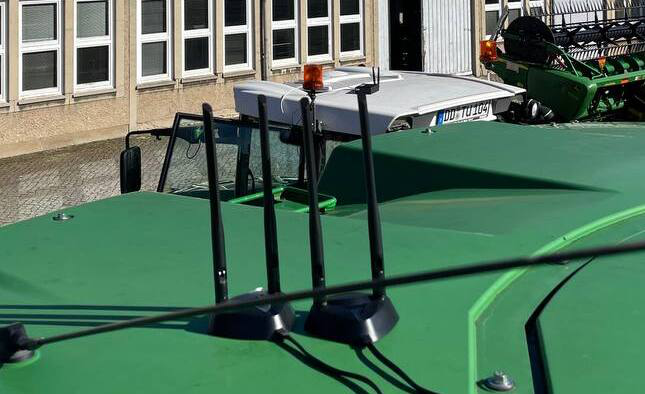
\includegraphics[width=0.98\textwidth]{figures/trainRun}
	\caption{Position of the Wi-Fi Devices on the \ac{TM} and the \ac{CH} during the trialrun}
	\label{fig:trailrunPositions}%
\end{figure}

\begin{figure}[H]%
	\centering
	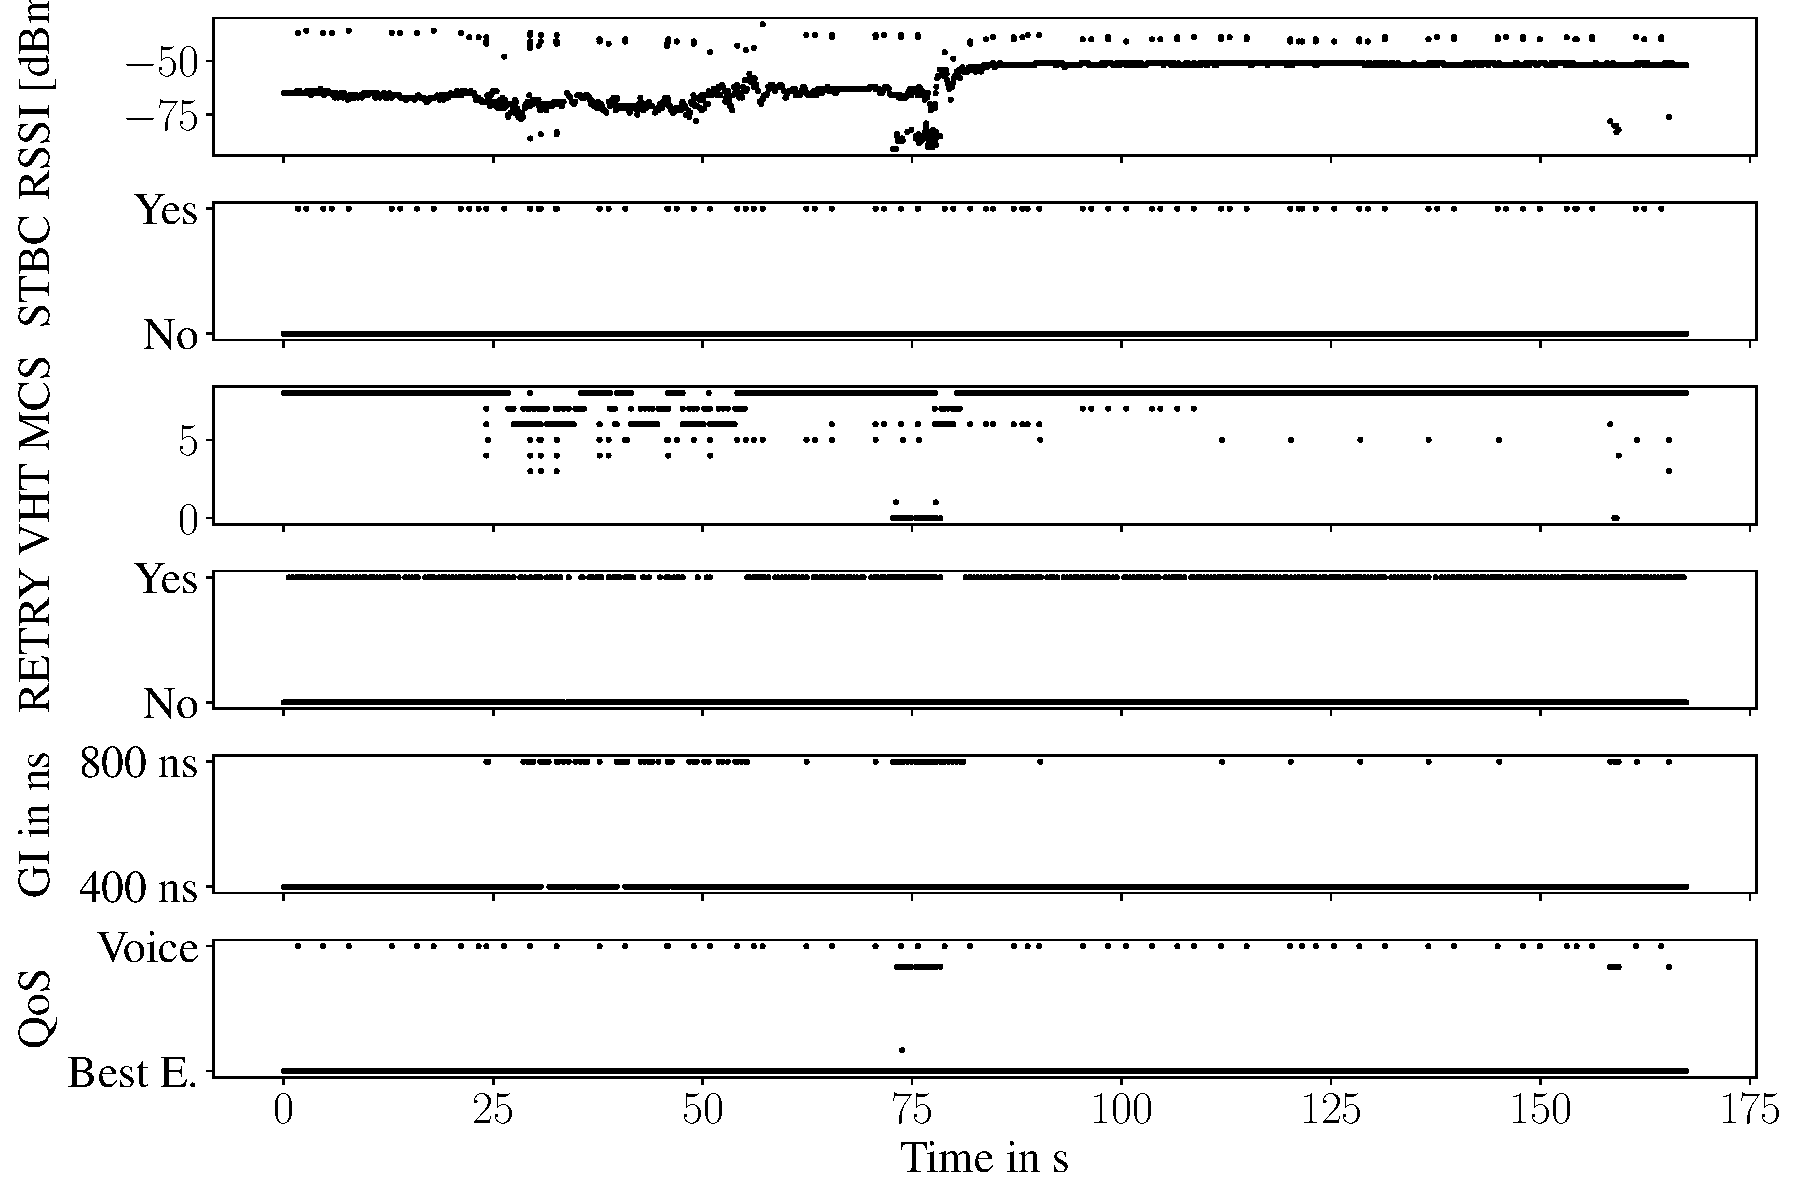
\includegraphics[width=0.98\textwidth]{figures/wireless5}
	\caption{All QoS data transmissions between the Wi-Fi \acf{AP} on the \acf{TM} and the Wi-Fi \ac{STA} on the \acf{CH} in a trialrun}
	\label{fig:trailrunAll}%
\end{figure}

\begin{figure}[H]%
	\centering
	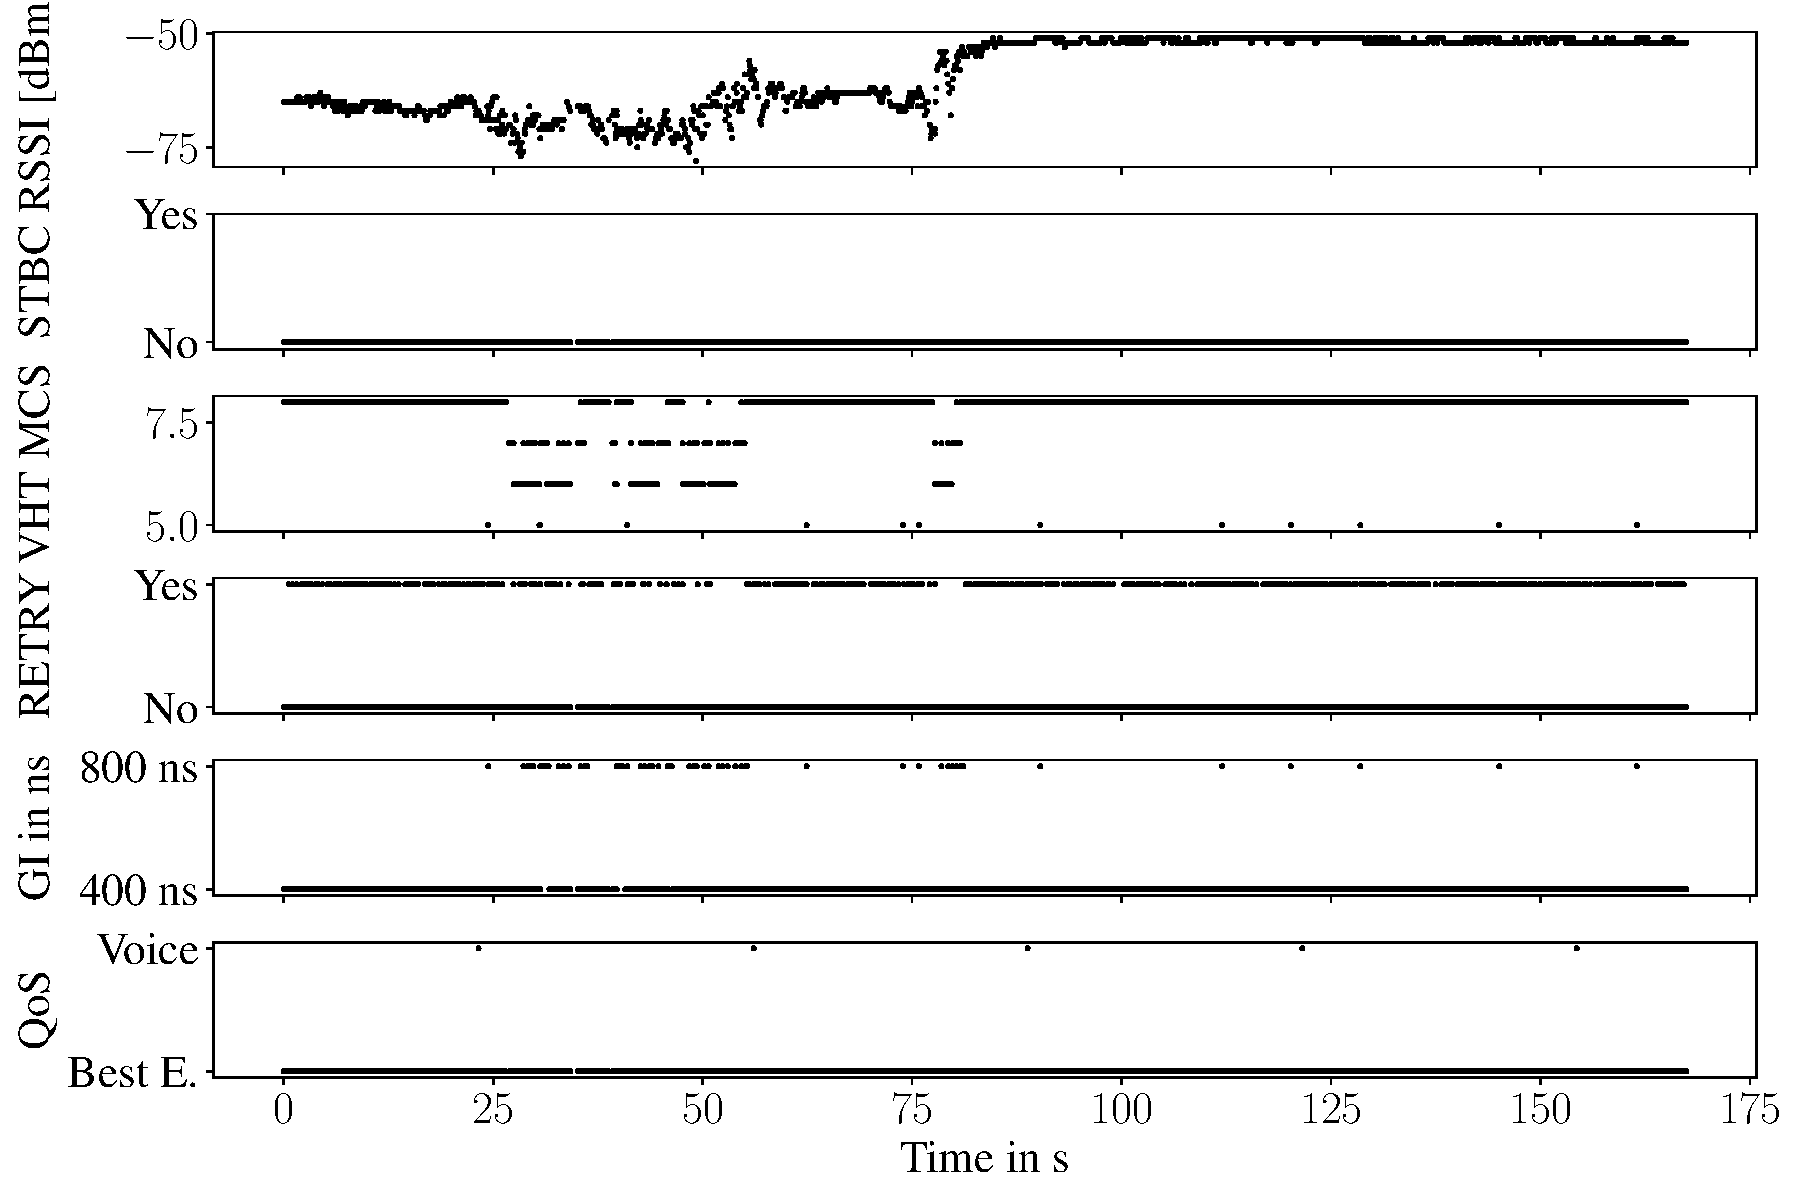
\includegraphics[width=0.98\textwidth]{figures/wireless5_lan}
	\caption{All QoS data transmissions between the Wi-Fi \acf{AP} on the \acf{TM} and the Wi-Fi \ac{STA} on the \acf{CH} in a trialrun,
	which were initiated by the iperf3 client on the \acf{TM}}
	\label{fig:trailrunIperf}%
\end{figure}

\begin{figure}[H]%
	\centering
	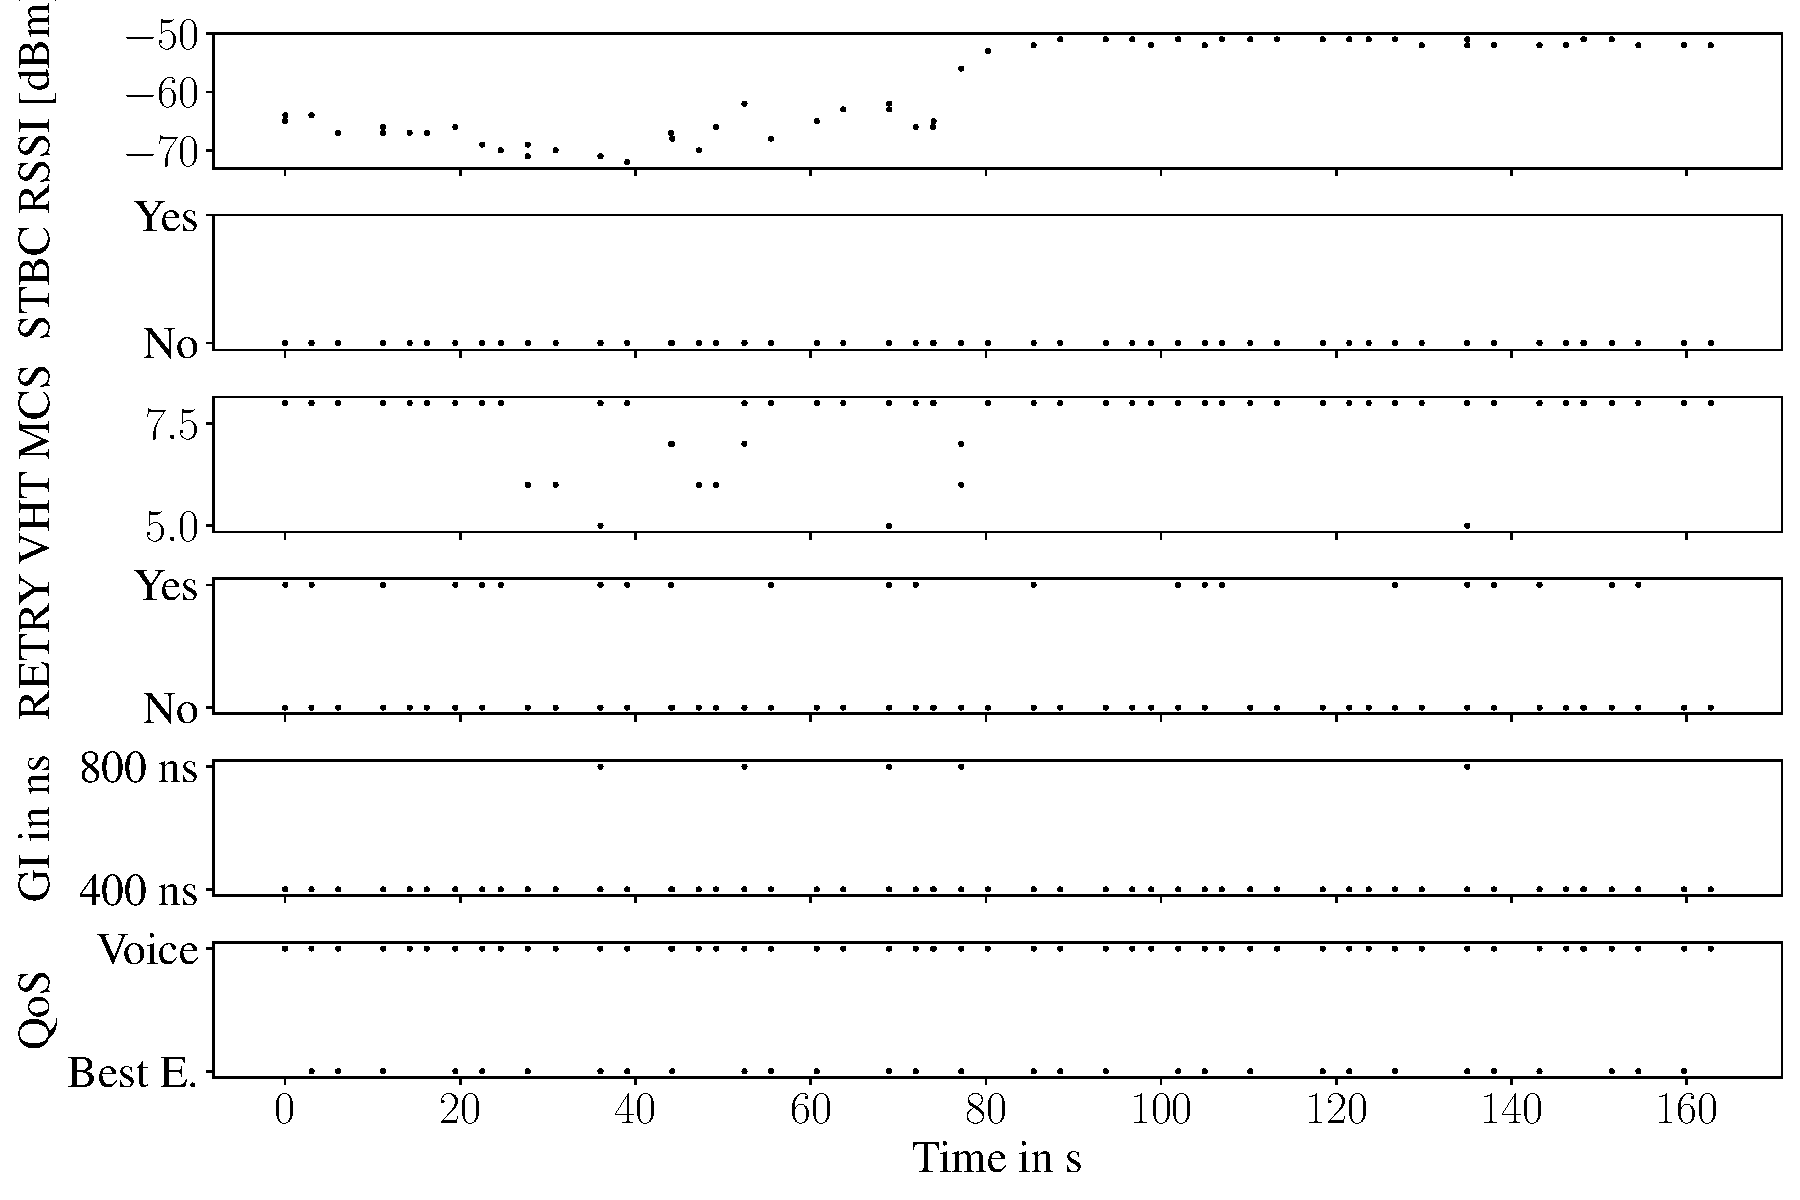
\includegraphics[width=0.98\textwidth]{figures/wireless5_ap}
	\caption{QoS data transmissions between the Wi-Fi \acf{AP} on the \acf{TM} and the Wi-Fi \ac{STA} on the \acf{CH} in a trialrun,
	which were initiated by \ac{AP}}
	\label{fig:trailrunAP}%
\end{figure}

\begin{figure}[H]%
	\centering
	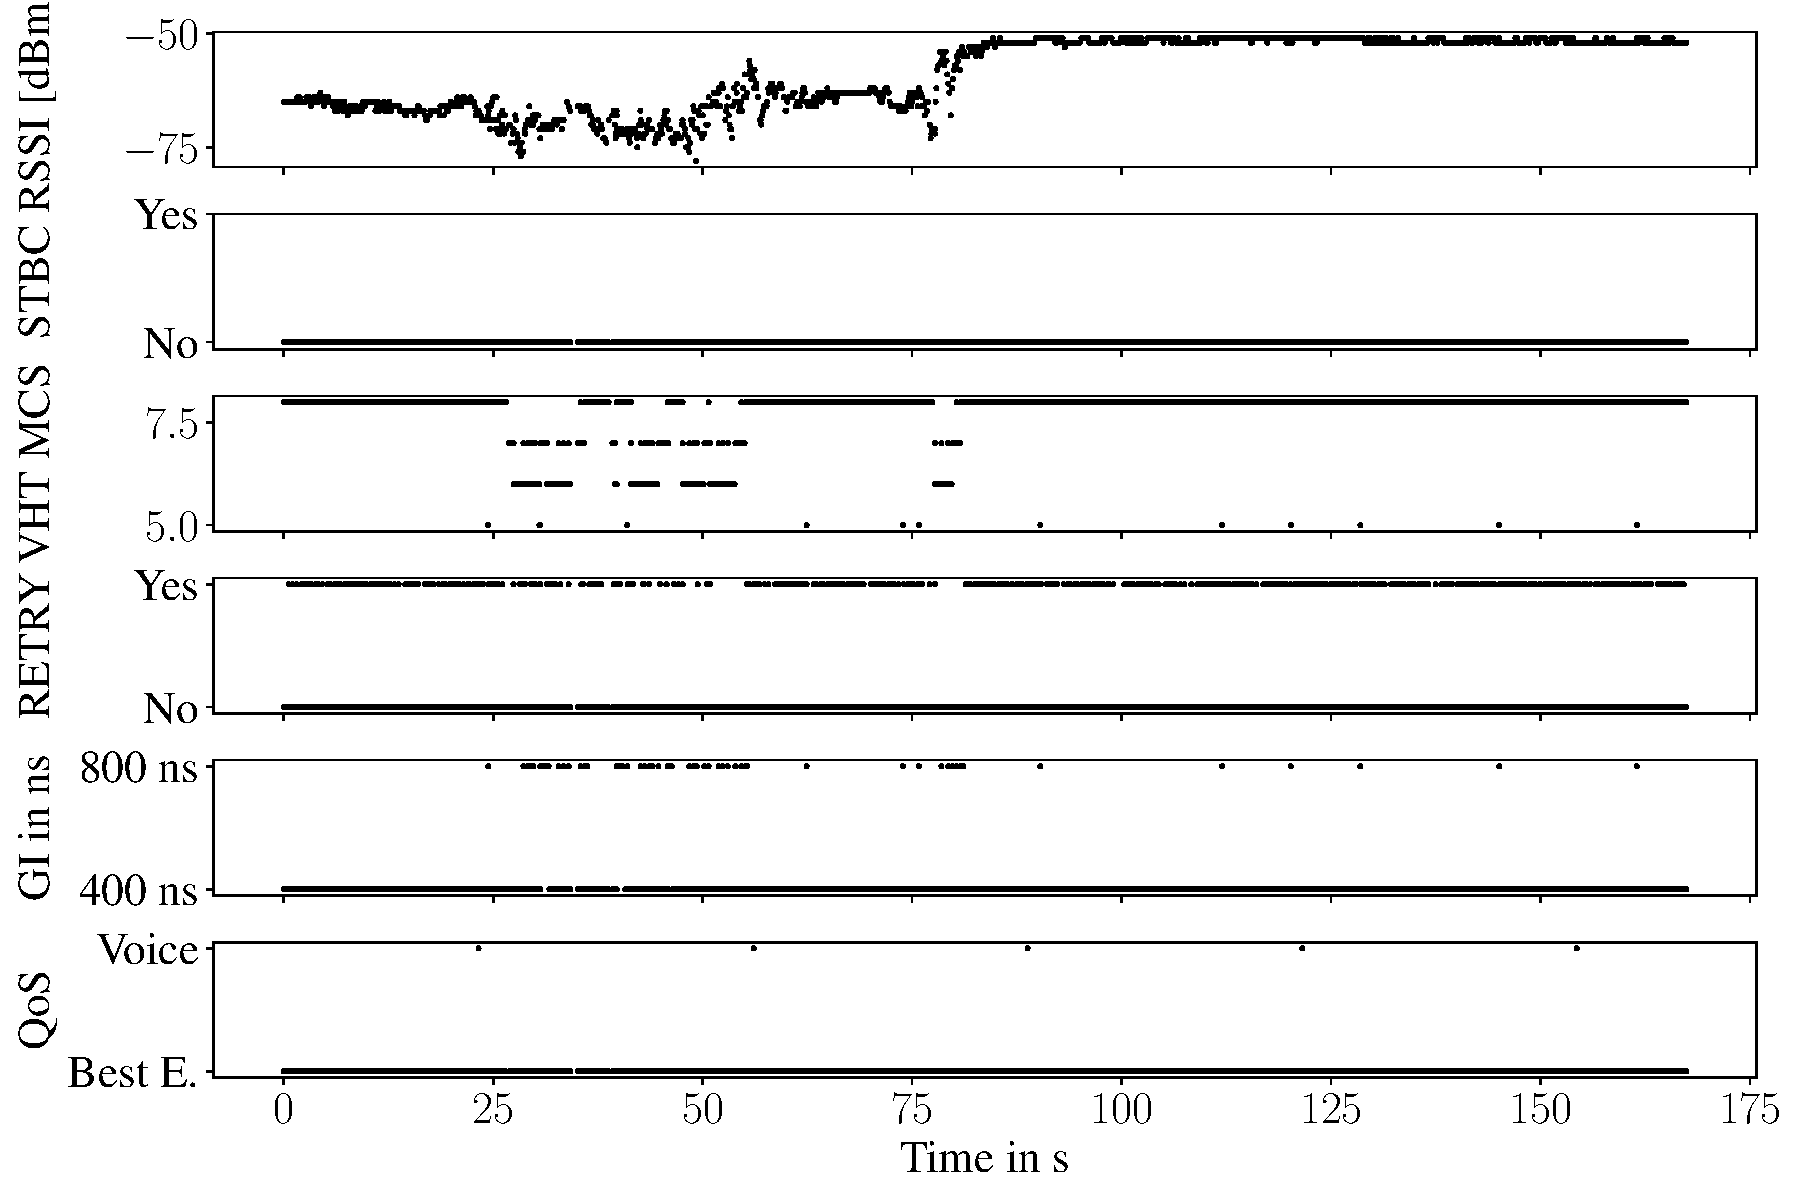
\includegraphics[width=0.98\textwidth]{figures/wireless5_lan}
	\caption{All QoS data transmissions between the Wi-Fi \acf{AP} on the \acf{TM} and the Wi-Fi \ac{STA} on the \acf{CH} in a trialrun,
	which were initiated by the Wi-Fi \ac{STA} on the \ac{CH}}
	\label{fig:trailrunNode}%
\end{figure}

\begin{figure}[H]%
	\centering
	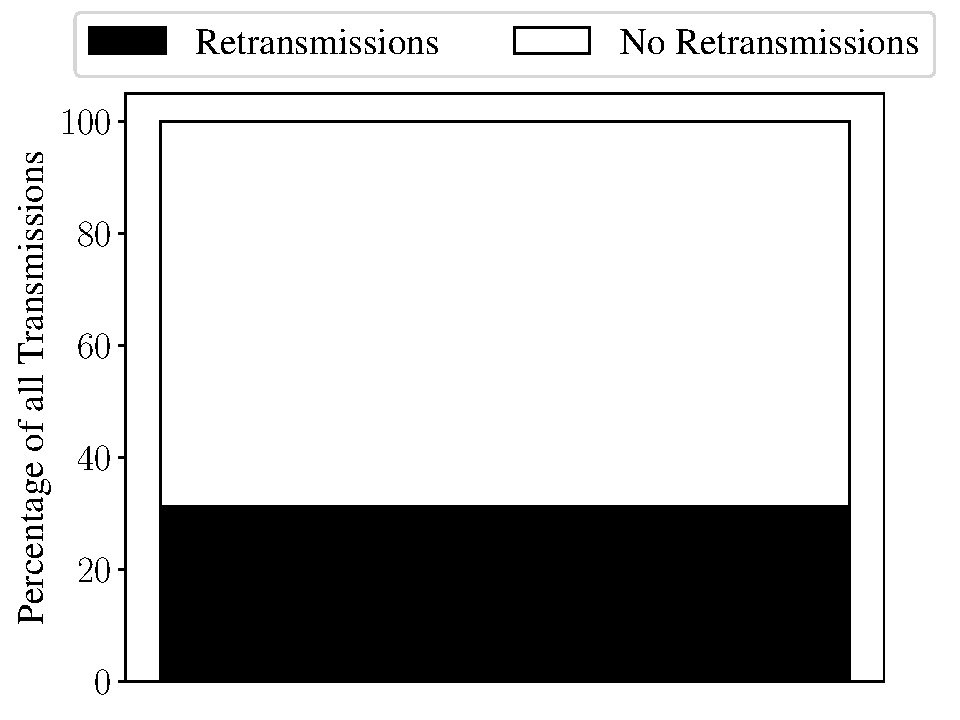
\includegraphics[width=0.8\textwidth]{figures/All_retries}
	\caption{Percentage of retransmissions for every transmission in the trialrun}
	\label{fig:retriesCount}%
\end{figure}

\todo[color=blue]{Den folgenden Output erhoffe ich mir. Den Text brauchst du als groben Übergang zum nächsten Abschnitt.}

The field experiment reveals that the Wi-Fi transmissions in the agricultural environment suffer from multipath effects which introduce
additional interferences.
Depending on the Wi-Fi physical layer configuration, the robustness of the transmissions is different and may result in a large number of retransmissions
as shown in \autoref{fig:retriesCount}.

In the following chapter, I will analyze which physical layer
configurations are suitable for the agricultural environment in order to establish a reliable communication,
which meets the requirements of data rate, range and latency.

